% !TeX root = ../../main.tex
% Add the above to each chapter to make compiling the PDF easier in some editors.

\chapter{Benchmark Setup}\label{ord:ch4}

% Basic Idea what is the benchmark about 
The established benchmark study is the centerpiece of this thesis and serves as main instrument to obtain insights about interactive segmentation methods.
In this study real participants apply the interactive methods introduced in Chapter \ref{ord:ch3}, in order to segment objects in various images.
The participating users are mostly employees of the company MVTec Software GmbH, located in Munich.
The participants have different levels of experience with labeling
Within this benchmark study the user interactions and the segmentation results are recorded and saved.

In total, \getNumberBenchmarkRuns \space runs of the benchmark study were performed, whereby \getNumberBenchmarkParticipants \space were completely unbiased participants and the remaining benchmark runs were performed by colleagues working on this topic.
A total of \getNumberBenchmarkAnnotations \space annotations were obtained.
Based on these observations the generalization capabilities of the methods are evaluated in Chapter \ref{ord:ch5}.
% real user label 
% Besides the application with real users also simulations are performed and used for evaluation, but they are not in the scope / part of the benchmakr)

% !TeX root = ../../main.tex
% Add the above to each chapter to make compiling the PDF easier in some editors.

\section{Benchmark Motivation}\label{ord:ch4:sec1}

% Motivation - title and research question
This benchmark study is motivated by the two main causes to evaluate real users and to use a diverse data set.
Both target to enable the evaluation on generalization capabilities of interactive segmentation methods.

First, the current evaluations of interactive methods feature the major drawback of using simulations.
The user input is created by simulations, instead of real users, as discussed in Section \ref{ord:ch2:sec3:subsec2}.
This measure seems reasonable with the amount of samples in test or validations sets used in the context of \gls{dl}.
However, these evaluations based on simulations are only meaningful to a limited extent, since a fundamental element, the user interaction, is not taken into account realistically.
% TODO Ref where an unrealistic user is simulated e.g., IOG
In simulations often an almost perfect user is simulated, that makes only few or none mistakes without any inaccuracies, which does not reflect reality.
In contrast, this benchmark study analyses the result of real participants, in order to obtain realistic insights on the models performance.
Thereby, the interaction of the users are recorded as described in Section \ref{ord:ch4:sec3}.
% TODO sure about this statement?
% An evaluation of the usability is especially valuable, because it is mostly not included in comparisons.
%TODO introduce the variance of different users here?


% Motivation Dataset
Second, the information value of an evaluation strongly depends on the used dataset.
The use of an unsuitable data set may lead to misrepresenting evaluation results.
% TODO ref PASCAL VOC section
To objectively evaluate the generalization capability of the interactive methods, a suitable dataset must be used.
For a data set to be suitable it must have a high variance in its samples.
In the context of image dataset this may be achieved by images with diverse domains and attributes.
Therefore, for the scope of this benchmark study a hand chosen dataset was created, which is further described in Section \ref{ord:ch4:sec2}.

% Reread confluence pages
% What is expected from the Benchmark
% !TeX root = ../../main.tex
% Add the above to each chapter to make compiling the PDF easier in some editors.

\section{Method Selection}\label{ord:ch4:sec2}

The benchmark study includes four methods to interactive create segmentation masks, as introduced in Chapter \ref{ord:ch3}. 
In the following their selection is reasoned.

Polygon drawing does not contain any smart algorithms, but just processes the user input.
This method is included, in order to establish a baseline, that realistically represents manual labeling.
Watershed transformation is included to represent the segmentation algorithms based on classical image processing.
With \gls{iog} and \gls{dextr} two \gls{dl} methods are part of the benchmark study, that represent the current state-of-the-art approaches.
Based on the comparison from Table \ref{tab:ch2:interactive-stae-of-the-art}, the \gls{iog} method performs best, by processing user clicks on fore- and background.
While the \gls{dextr} method only processed user clicks on the boundary of the object.

In order to keep the scope of this thesis feasible, the benchmark study contains these four interactive segmentation methods.

% !TeX root = ../../main.tex
% Add the above to each chapter to make compiling the PDF easier in some editors.

\section{Benchmark Statistics}\label{ord:ch4:sec3}

In the scope of the benchmark study several statistics were recorded and measured, that may be grouped in three parts: segmentation result, user interactions and, user survey.

% #1 Performance IoU
First, the saved segmentation results are used to calculate the \gls{iou} as measure of performance for each user created annotation.

% #2 User interactions.
Second, the user interactions were recorded, that are required to perform the interactive methods.
% TODO what about usability??
% Based on these statistics the usability of the labeling process is evaluated.
These statistics on the user interactions exist for every annotation, the most important are presented in the following:
\begin{itemize}
	\item \textbf{Used method}, the interactive method used to create the annotation.
	\item \textbf{Annotation time}, the time spent to create the annotation.
	\item \textbf{Number of clicks}, the number of clicks used.
	\item \textbf{Number of strokes}, the amount of strokes drawn for the annotation.
	\item \textbf{Stroke time}, the time spent on each stroke, in order to differentiate between short and long strokes.
	\item \textbf{Number of foreground clicks}, the amount of clicks on the foreground.
	\item \textbf{Number of background clicks}, the amount of clicks on the background.
	% image_time
	% image_id
	% single_methods
	% single_box_times
	% single_mask_times
	% single_hole_time
	% single_clicks
	% single_strokes
	% single_stroke_times
	% single_change_box_time
	% single_change_mask_time
	% single_change_clicks
	% single_change_strokes
	% single_change_strokes_times
	% fg_click_row
	% fg_click_col
	% num_fg_clicks
	% idx_fg_clicks
	% bg_click_row
	% bg_click_col
	% num_bg_clicks
	% idx_bg_clicks
	% bbox_click_row1
	% bbox_click_col1
	% bbox_click_row2
	% bbox_click_col2
	% idx_bbox_clicks
	% fg_click_region
	% bg_click_region
	
\end{itemize}

% #3 Survey to get an idea about the soft factors.
Third, the participants filled out a survey, after completing the benchmark study.
This survey enables an insight on the usability of the methods, that are not measurable.

% TODO table that provides insights on the pandas datarfame
% !TeX root = ../../main.tex
% Add the above to each chapter to make compiling the PDF easier in some editors.

\section{Image Selection}\label{ord:ch4:sec4}

As the importance of a suitable dataset is already highlighted, this Section focuses on the composition of the benchmark dataset.
It was a conscious decision to select images from different domains and with different attributes.
Both, diverse domains and attributes, are fundamental to evaluate the generalization capability of the methods.
The selection of images for the dataset was done manually.
Thereby, images from various datasets are included: sPASCAL \gls{voc} \cite{Eve20-PascalVOC}, COCO \cite{Lin14-Coco}, DAVIS \cite{Per16-DAVIS}, CityScapes \cite{Cor16-Cityscapes}, \gls{d2s} \cite{Paddo18-D2S}, \gls{mad} \cite{Bergmann19-MAD}, MVTec Screws \cite{UFN19-Screws}, and other unpublished datasets from the MVTec Software GmbH.
% Other unpublsished MVTec Datasets
%--- pill_bags
%--- MVTec segmentation and counting dataset
%--- Single images: Cans, Cigarettes, Cereals
%--- MVTec closed packed & occluded object detection dataset (CPOD)
% Nachlabeln von Bildern
For some images from open source datasets the \gls{gt} was improved, in order to achieve a consistent goodness of the \gls{gt} for the benchmark dataset.
% TODO appendix with various examples of the image selection?

% Amount of images
The benchmark dataset contains 87 images with 225 annotations.
% Vergleichsweise klein
In the context of \gls{dl}, this evaluation datasets is comparatively small.
It was kept small on purpose, to enable users to label the majority of the images in a reasonable expenditure of time.
 
% es gibt kein 'perfektes' Dataset -> always depends on the porpuse of the model
It should be highlighted, that there is no \textit{ultimate} evaluation dataset, because the suitability of a dataset depends on the objective of the task.
Within the scope of this thesis, the main objective is to evaluate the generalization capabilities of interactive segmentation methods by real users.
The established dataset fulfills this evaluation purpose, as described in Chapter \ref{ord:ch5}.


\subsection{Domains}\label{ord:ch4:sec2:subsec1}

In order to ensure the variety of the benchmark dataset, each image was categorized into one of four domains:
%
\begin{itemize}
	\item \textbf{Standard}, contains casual objects and scenes, that are common in daily life.
	The images mostly origin from \textit{general-use} datasets as PASCAL \gls{voc}, COCO, and DAVIS.
	\item \textbf{Urban}, represents images of urban road scenes as in CityScapes.
	\item \textbf{Industrial}, focuses on images from an industrial context, that are usually underrepresented in  \textit{general-use} datasets.
	Images from \gls{d2s}, MVTec Screws and other unpublished dataset are included.
	\item \textbf{Anomaly}, contains images from the \gls{mad} dataset, which originally was used for anomaly detection.
	These images contain objects with defects such as cracks, contaminations, or holes.
\end{itemize}

% State of the art
\begin{table}[h!]
	\centering
	\begin{tabular}{l|c|c|c|c}
		Domain				& Standard & Urban & Industrial & Anomaly \\
		\hline
		Number of images 	& - & - & - & - \\
		Number of object 	& - & - & - & - \\
	\end{tabular}
	\caption[tbd.]{
		tbd.
		} \label{tab:ch4:domains_overview}
\end{table}

\subsection{Attributes}\label{ord:ch4:sec2:subsec2}

The attributes of the benchmark images and objects also have a great impact on the segmentation and evaluation.
To further evaluate their effect and how well the methods generalize, the following attribute categories have been established and assigned for each image.
% TODO Comment von Paddo - Werden die überhaupt verwendet? Bitte angeben falls nicht!

\begin{itemize}
	\item \textbf{Illumination}, states if an image is underexposed, overexposed, or normal.
	\item \textbf{Color channel}, differentiates between \gls{rgb} and gray scale images.
	\item \textbf{Contrast}, states if the contrast in the image is high or low.
	\item \textbf{Shapes}, describes the shape of the object as convex, uneven, or if it contains holes.
	\item \textbf{Overlap}, states if multiple objects are touching, overlapping, or there is no contact at all.
	\item \textbf{Number of objects}, gives a simplified idea about the amount of objects in the image (single, few, or many).
	\item \textbf{Error type}, describes the type of error for images of the domain \textit{anomaly}.
	The error types categories are \textit{holes}, \textit{cracks}, \textit{contamination} or \textit{none} as default. 
	\item \textbf{Reflection}, binary describes if the objects are reflecting.
	\item \textbf{Background texture}, describes the background of the image as plain, textured or cluttered.
	\item \textbf{Foreground texture}, describes the foreground of the image as plain, textured or cluttered.
	% TODO decide if to remove some attributes if they are not used in the evaluation anyway.
\end{itemize}

% TODO Comment von Paddo - Sowohl für Attributes als auch Domains wäre eine Tabelle ganz nett wo man sieht wieviele Bilder den Attributen zugeordnet wurden.
% !TeX root = ../../main.tex
% Add the above to each chapter to make compiling the PDF easier in some editors.

\section{Benchmark Procedure}\label{ord:ch4:sec5}
% 
The benchmark study is realized within a label tool, that was implemented in the scope of this thesis in the integrated development environment \textit{HDevelop} from MVTec.
Within the labeltool also the four interactive methods are implemented.
The collection of the benchmark statistics is also realized within this program.
The labeltool provides a user interface with various windows as shown in Figure \ref{fig:ch4:sec4:labeltool}.

% Introduction for each participants.
The participants got an introduction to the labeltool, before they started.
% 'Do as long as you want'-policy
The time spent for the participation in the benchmark varied between the users, due to their available working time. % company time.
The average participant created 72.4 annotations in 63 minutes.
% Random order of the images to enable an equal coverage of all images
Therefore, for each benchmark user the images were arranged randomly, in order to ensure a uniform coverage of the images.

% Label task.
The task of the participant is to create a segmentation mask for the single objects in the image.
To create a mask, one of the four interactive methods needs to be applied.
% Free choice of methods.
The user can choose which method to apply.
Thereby, statistics on the same object are obtained, that are created by various methods.
Further, the participation in the benchmark study was kept interesting, by giving the participants a free choice which method to choose.
% Label RoI.
The task to label each object was limited to the objects inside a turquoise polygon, that is referred to as label region, as illustrated in Figure \ref{fig:ch4:sec4:labeltool}.
Thereby, not all objects in an image should be labeled, in order to realize a reasonable participation time.
It is not part of the user's task to assign a class name for the created annotation.
% Label instructions
An additional label instruction was provided partially, to clarify the scope and avoid misunderstandings.

\begin{figure}
	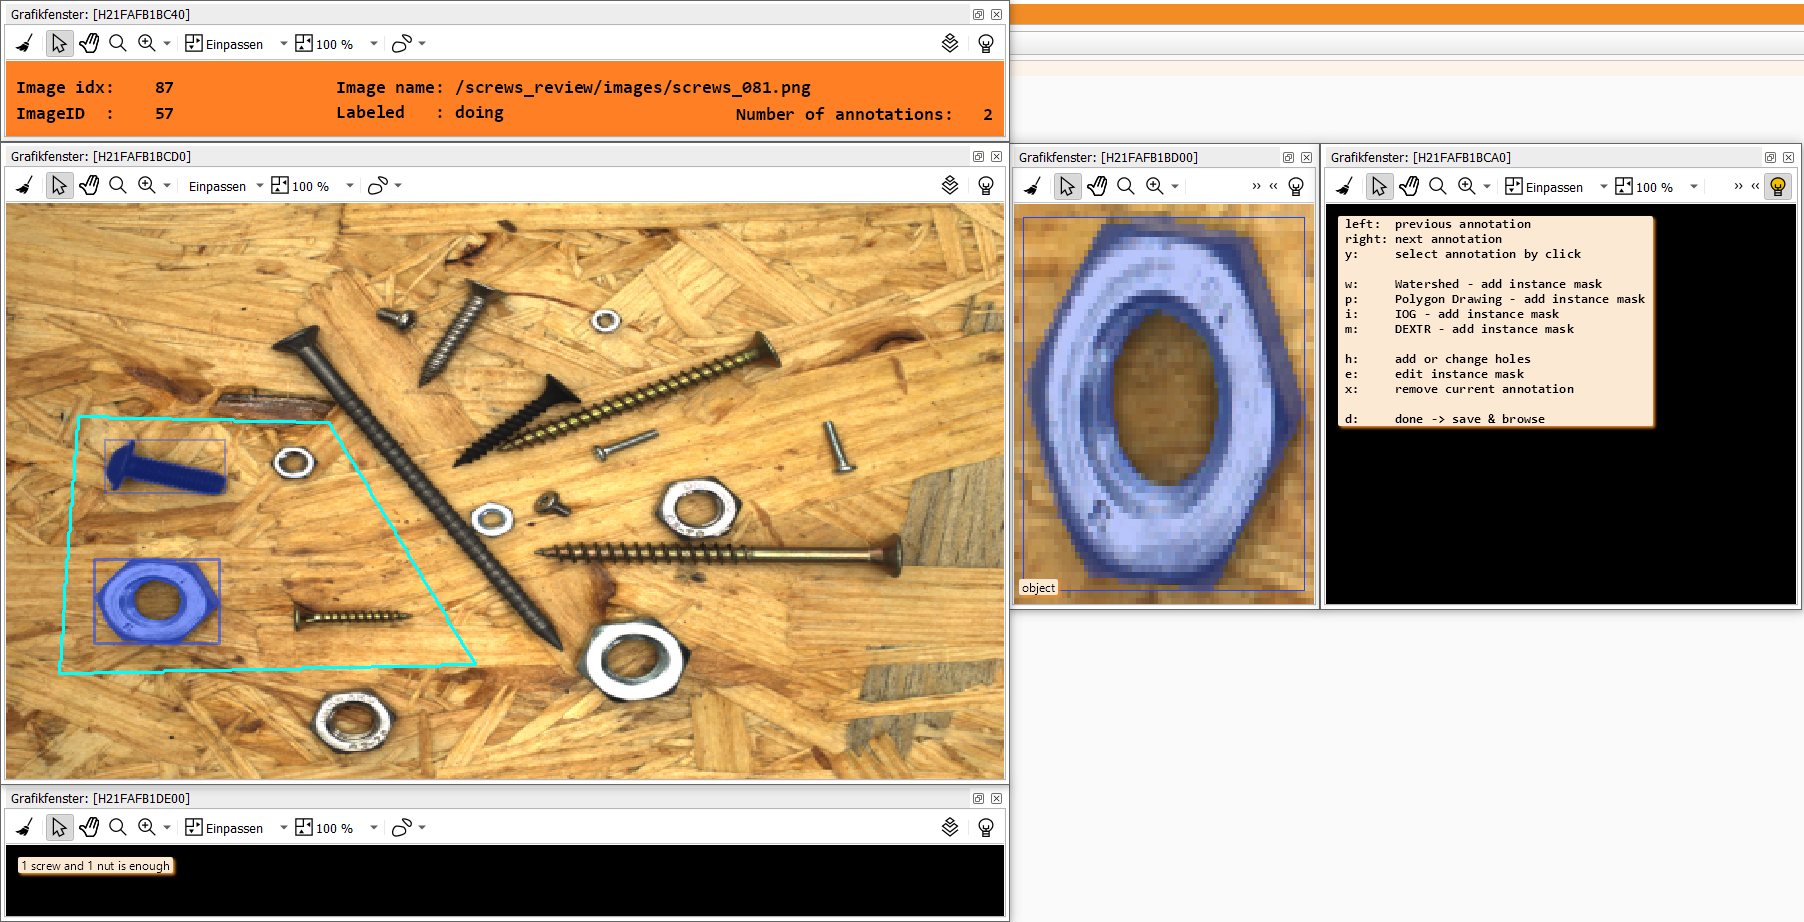
\includegraphics[width=\linewidth]{figures/chap45_labeltool_scrennshot.png}
	\caption[Screenshot of the user interface from the labeltool]{		
		Screenshot of the user interface from the labeltool implemented in HDevelop.
		The image origins from the MVTec Screws Dataset.
		It contains two annotation masks colored in blue and the label region as turquoise colored polygon.
		The smaller image window displays the currently selected annotation zoomed in.
		The window on the right, presents the user with the available options and the corresponding control key.
		On the bottom is a small window with a label instruction.
	}
	\label{fig:ch4:sec4:labeltool}
\end{figure}
